%%%%%%%%%%%%%%%%%%%%%%%%%%%%%%%%%%%%%%%%%%%%%%%%%%%%%%%%%%%%%%%%%%%%%%%%%%%%% %
% social-media.tex
%
% Ian Roberts, May 2014
%
% $Id: uima.tex,v 1.3 2006/10/21 11:44:47 ian Exp $
%
%%%%%%%%%%%%%%%%%%%%%%%%%%%%%%%%%%%%%%%%%%%%%%%%%%%%%%%%%%%%%%%%%%%%%%%%%%%%%


%%%%%%%%%%%%%%%%%%%%%%%%%%%%%%%%%%%%%%%%%%%%%%%%%%%%%%%%%%%%%%%%%%%%%%%%%%%%%
\chapt[chap:social]{Tools for Social Media Data}
\markboth{Tools for Social Media Data}{Tools for Social Media Data}
%%%%%%%%%%%%%%%%%%%%%%%%%%%%%%%%%%%%%%%%%%%%%%%%%%%%%%%%%%%%%%%%%%%%%%%%%%%%%
\nnormalsize

Social media provides data that is highly valuable to many organizations, for
example as a way to track public opinion about a company's products or to
discover attitudes towards ``hot topics'' and breaking news stories.  However,
processing social media text presents a set of unique challenges, and text
processing tools designed to work on longer and more well-formed texts such as
news articles tend to perform badly on social media.  To obtain reasonable
results on short, inconsistent and ungrammatical texts such as these requires
tools that are specifically tuned to deal with them.

This chapter discusses the tools provided by GATE for use with social media
data.

%%%%%%%%%%%%%%%%%%%%%%%%%%%%%%%%%%%%%%%%%%%%%%%%%%%%%%%%%%%%%%%%%%%%%%%%%%%%%
\sect[sec:social:twitter]{Tools for Twitter}

The Twitter tools in GATE are provided in two plugins.  The
\verb!Format_Twitter! plugin contains tools to load and save documents in GATE
using the JSON format provided by the Twitter APIs, and the \verb!Twitter!
plugin contains a tokeniser and POS tagger tuned to Tweets, a tool to split
up multi-word hashtags, and an example named entity recognition application
called {\em TwitIE} which demonstrates all these components working together.
The \verb!Twitter! plugin makes use of PRs from the \verb!Stanford_CoreNLP!
plugin, which will be loaded automatically when the \verb!Twitter! plugin is
loaded.

%%%%%%%%%%%%%%%%%%%%%%%%%%%%%%%%%%%%%%%%%%%%%%%%%%%%%%%%%%%%%%%%%%%%%%%%%%%%%
\sect[sec:social:twitter:format]{Twitter JSON format}
%%%%%%%%%%%%%%%%%%%%%%%%%%%%%%%%%%%%%%%%%%%%%%%%%%%%%%%%%%%%%%%%%%%%%%%%%%%%%
%
Twitter provides APIs to search for Tweets according to various criteria, and
to collect streams of Tweets in real-time.  These APIs return the Tweets in a
structured JSON format%
\footnote{\url{https://dev.twitter.com/docs/platform-objects/tweets}} which
includes the text of the Tweet plus a large amount of supporting metadata.
The GATE \verb!Format_Twitter! plugin contains a format analyser for this JSON format
which allows you to load a file of one or more JSON Tweets into a GATE
document.  The format analyser can handle multiple Tweets in one file,
represented as any of:
\begin{itemize}
\item a top-level JSON array \verb![{...},{...}]!
\item a top-level JSON object containing properties ``search\_metadata'' and
  ``statuses'', where the ``statuses'' property is an array of Tweets (this is
  the format returned by a call to Twitter's ``search'' API)
\item or simply concatenated together, optionally with white space or newline
  characters between adjacent objects (this is the format returned by Twitter's
  streaming APIs).
\end{itemize}
Loading the plugin registers the
document format with GATE, so that it will be automatically associated with
files whose names end in ``\verb!.json!''; otherwise you need to specify
\verb!text/x-json-twitter! for the document mimeType parameter.  This will work
both when directly creating a single new GATE document and when populating a
corpus.

Each tweet object's \verb!text! value is converted into the document
content\footnote{HTML entity references \texttt{\&amp;}, \texttt{\&lt;} and
\texttt{\&gt;} are decoded into the corresponding characters},
which is covered with a \emph{Tweet} annotations whose features represent
(recursively when appropriate, using \emph{Map} and \emph{List}) all the other
key-value pairs in the tweet object.  \textbf{Note:} these recursive values are
difficult to work with in JAPE; the special corpus population tool described
next allows important key-sequences to be ``brought up'' to the document content
and the top level of the annotation features.  Any entities described by the
standoff markup ``entities'' JSON property will be converted into their
corresponding GATE annotations (see below for details).

Multiple tweet objects in the same JSON file are separated by blank lines (which
are not covered by \emph{Tweet} annotations).

As well as the document format parser to load Tweets into a single GATE
document, the plugin provides a ``Populate from Twitter JSON files'' option on
the GATE Corpus right-click menu.  Selecting this option bringgs up a dialog
that allows you to select one or more files of tweets in the Twitter API's JSON
format and set the following options to populate the corpus.
%%
\begin{description}
\item[Encoding]  The default here is UTF-8 (regardless of your Java default) to
  conform to Twitter JSON.
\item[One document per tweet] If this box is ticked (the default), each tweet
  will produce a separate document.  If not, each {\em input file} will produce
  one GATE document.
\item[Annotations for ``entities''] If this box is ticked (the default), any
  entities described by the standoff markup ``entities'' JSON property will be
  converted into their corresponding GATE annotations (see below).
\item[Content keys] The values of these JSON keys are converted into strings and
  concatenated into each tweet's document content.  Colon-delimited strings
  specify nested keys, e.g., ``\texttt{user:name}'' will yield the value of the
  \texttt{name} key in the map that is the value of the \texttt{user} key.
  Missing key sequences are ignored.  Each span of text will be covered by an
  annotation whose type is the key sequence.
\item[Feature keys] The key sequences and values of these JSON keys (where
  present) are turned into feature names and values on the tweet's main
  \texttt{Tweet} annotation.
\item[Save configuration] This button saves the current options in an XML file
  for re-use later.
\item[Load configuration] This button sets the options according to a saved XML
  configuration.
\end{description}
%%
Again, the input can be in any of the three formats discussed above (an array
of Tweets, a search result, or a stream of concatenated objects).
Every tweet in the resulting GATE documents is covered by a \texttt{Tweet}
annotation with features specified by the ``feature keys'' option.  Multiple
tweets in the same GATE document are separated by a blank line (two newlines).

Corpus population from Twitter JSON files is also accessible programmatically
when this plugin is loaded, using the public static void method
\texttt{gate.corpora.twitter.Population.populateCorpus(final Corpus corpus, URL
  inputUrl, String encoding, List<String> contentKeys, List<String> featureKeys,
  int tweetsPerDoc, boolean processEntities)}.

\subsect[sec:social:twitter:entities]{Entity annotations in JSON}

Twitter's JSON format provides a mechanism to represent annotations over the
Tweet text as standoff markup, via a JSON property named ``entities''.  The
value of this property is an object with one property for each entity
\emph{type}, whose value is a list of objects representing the individual
annotations.  Within each individual entity object, the ``indices'' property
gives start and end character offsets of the annotation within the Tweet text.

\begin{verbatim}
{
  "text":"@some_user this is a nice #example",
  "entities":{
    "user_mentions":[
      {
        "indices":[0,10],
        "screen_name":"some_user",
        ...
      }
    ],
    "hashtags":[
      {
        "indices":[26,34],
        "text":"example"
      }
    ]
  }
}
\end{verbatim}

Both the single document format parser and the corpus population tool are able
to convert this structure into GATE annotations.  The entity type (e.g.
\verb!user_mentions!) becomes the annotation type, the \verb!indices!  property
provides the offsets, and the other properties become features of the generated
annotation.

By default, the entity annotations are created in the ``Original markups''
annotation set, as is the usual convention for annotations generated by a
document format.  However, if the entity type contains a colon character (e.g.
\verb!"Key:Person":[...]!) then the portion before the colon is taken to be an
annotation set name and the portion after the colon is the annotation type (in
this example, a ``Person'' annotation in the ``Key'' annotation set).  An
empty annotation set name (i.e. \verb!":Person"!) creates the corresponding
annotations in the default annotation set.  This scheme is designed to be
compatible with the GATE JSON export mechanism described in the next section.

%%%%%%%%%%%%%%%%%%%%%%%%%%%%%%%%%%%%%%%%%%%%%%%%%%%%%%%%%%%%%%%%%%%%%%%%%%%%%
\sect[sec:social:twitter:export]{Exporting GATE documents as JSON}

Loading the \verb!Format_Twitter! plugin also adds a ``GATE JSON'' option to the
``Save as\ldots'' right-click menu on documents and corpora, to export GATE
documents in the Twitter-style JSON format.  This tool can save a document or
corpus of documents as a single file where each Tweet in the document or corpus
is represented as a JSON object, and the set of objects are represented either
as a single top-level JSON array (\verb![{...},{...}]!) or simply as one object
per line (as per Twitter's streaming APIs).  This exporter can be used for any
GATE document, not just for documents that were initially loaded from Twitter
JSON format, and can be used as a much more compact alternative to GATE XML, or
as an easy-to-parse interchange format to pass GATE-annotated documents to
non-GATE tools.

The format is the same as Twitter's -- the text becomes a property ``text'' in
the JSON, and annotations are represented as standoff markup in the
``entities'' property, which is an object whose keys are annotation types and
whose corresponding values are arrays of objects representing the annotations.

\begin{figure}[htb]
  \centering
  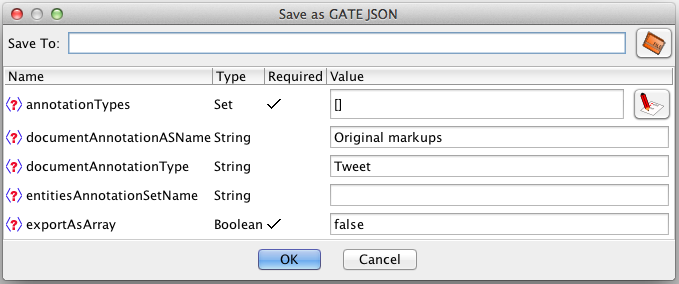
\includegraphics[width=0.8\textwidth]{save-as-json.png}
  \caption{Options dialog for saving a document or corpus as JSON}
  \label{fig:social:save-as-json}
\end{figure}

The available options for the JSON exporter are shown in
figure~\ref{fig:social:save-as-json}.  In detail, they are:
\begin{description}
\item[documentAnnotationASName/documentAnnotationType] the annotation set and
  type that should be treated as covering each span of text that should be output
  as a separate JSON object.  By default this is annotations of type ``Tweet'' in
  the ``Original markups'' set (i.e. the annotations covering individual Tweets
  parsed by the JSON document format parser or corpus population tool).  If a
  document contains any annotations of the specified type then one JSON object
  will be output for each such annotation $X$, with the text and entity
  annotations constrained to the span of $X$.  In addition, features of $X$
  will become top-level properties of the resulting JSON object.  Text that is
  not covered by any such annotation will not be saved.  If there are no
  document annotations found in a particular document (or if the
  documentAnnotationType parameter is unset) then the whole of the document
  text will be output as a single JSON object.
\item[entitiesAnnotationSetName] the primary annotation set that should be
  scanned for entity annotations.
\item[annotationTypes] the entity annotation types to output.
\item[exportAsArray] if true, output the objects as a top-level JSON array.  If
  false (the default), output the JSON objects directly at the top level,
  separated by newlines.
\end{description}

Annotation types to be saved can be specified in two ways.  Plain annotation
type names such as ``Person'' will be taken from the specified
\emph{entitiesAnnotationSetName}, but if a type name contains a colon character
(e.g. ``Key:Person'') then the portion before the colon is treated as the
annotation set name and the portion after the colon as the annotation type.
The full name including the colon will be used as the type label in the
``entities'' object, so if the resulting JSON were re-loaded into GATE the
annotations would be re-created in the same annotation sets they originally
came from.

%%%%%%%%%%%%%%%%%%%%%%%%%%%%%%%%%%%%%%%%%%%%%%%%%%%%%%%%%%%%%%%%%%%%%%%%%%%%%
\sect[sec:social:twitter:prs]{Low-level PRs for Tweets}

The \verb!Twitter! plugin provides a number of low-level language processing
components that are specifically tuned to Twitter data.

The ``Twitter Tokenizer'' PR is a specialization of the ANNIE English Tokeniser
for use with Tweets.  There are a number of differences in the way this
tokeniser divides up the text compared to the default ANNIE PR:
%
\begin{itemize}
\item URLs and abbreviations (such as ``gr8'' or ``2day'') are treated as a
  single token.
\item User mentions (\verb!@username!) are two tokens, one for the \verb!@! and
  one for the username.
\item Hashtags are likewise two tokens (the hash and the tag), but see below
  for another component that can split up multi-word hashtags.
\item ``Emoticons'' such as \verb!:-D! can be treated as a single token.  This
  requires a gazetteer of emoticons to be run before the tokeniser, an example
  gazetteer is provided in the Twitter plugin. This gazetteer also normalises
  the emoticons to help with classification, machine learning etc. For example,
  \verb!:-D!, and \verb!8D! are both normalized to \verb!:D!.
\end{itemize}

The ``Tweet Normaliser'' PR uses a spelling correction dictionary to correct
mis-spellings and a Twitter-specific dictionary to expand common abbreviations
and substitutions.  It replaces the \verb!string! feature on matching tokens
with the normalised form, preserving the original string value in the
\verb!origString! feature.

The ``Twitter POS Tagger'' PR uses the Stanford Tagger
(section~\ref{sec:misc:creole:stanford}) with a model trained on Tweets.  The
POS tagger can take advantage of expanded strings produced by the normaliser
PR.

%%%%%%%%%%%%%%%%%%%%%%%%%%%%%%%%%%%%%%%%%%%%%%%%%%%%%%%%%%%%%%%%%%%%%%%%%%%%%
\sect[sec:social:twitter:hashtag]{Handling multi-word hashtags}

When rendering a Tweet on the web, Twitter automatically converts contiguous
sequences of alpha-numeric characters following a hash (\verb!#!) into links
to search for other Tweets that include the same string.  Thus ``hashtags''
have rapidly become the de-facto standard way to mark a Tweet as relating to a
particular theme, event, brand name, etc.  Since hashtags cannot contain white
space, it is common for users to form hashtags by running together a number of
separate words, sometimes in ``camel case'' form but sometimes simply all in
lower (or upper) case, for example ``\#worldgonemad'' (as search queries on
Twitter are not case-sensitive).

The ``Hashtag Tokenizer'' PR attempts to recover the original discrete words
from such multi-word hashtags.  It uses a large gazetteer of common English
words, organization names, locations, etc. as well as slang words and
contractions without the use of apostrophes (since hashtags are alphanumeric,
words like ``wouldn't'' tend to be expressed as ``wouldnt'' without the
apostrophe).  Camel-cased hashtags (\verb!#CamelCasedHashtag!) are split at
case changes.

More details, and an example usecase, can be found in \cite{Maynard14a}.

%%%%%%%%%%%%%%%%%%%%%%%%%%%%%%%%%%%%%%%%%%%%%%%%%%%%%%%%%%%%%%%%%%%%%%%%%%%%%
\sect[sec:social:twitie]{The TwitIE Pipeline}

The Twitter plugin includes a sample ready-made application called TwitIE,
which combines the PRs described above with additional resources borrowed from
ANNIE and the TextCat language identification PR to produce a general-purpose
named entity recognition pipeline for use with Tweets.  TwitIE includes the
following components:

\begin{itemize}
\item Annotation Set Transfer to transfer Tweet annotations from the Original
  markups annotation set.  For documents loaded using the JSON document format
  or corpus population logic, this means that each Tweet will be covered by a
  separate Tweet annotation in the final output of TwitIE.
\item \emph{Language identification} PR (see
  section~\ref{sec:misc-creole:language-identification}) using language models
  trained on English, French, German, Dutch and Spanish Tweets.  This creates a
  feature \verb!lang! on each Tweet annotation giving the detected language.
\item \emph{Twitter tokenizer} described above, including a gazetteer of
  emoticons.
\item \emph{Hashtag tokenizer} to split up hashtags consisting of multiple
  words.
\item The standard ANNIE \emph{gazetteer} and \emph{sentence splitter}.
\item \emph{Normaliser} and \emph{POS tagger} described above.
\item Named entity JAPE grammars, based largely on the ANNIE defaults but with
  some customizations.
\end{itemize}

Full details of the TwitIE pipeline can be found in \cite{bontcheva2013twitie}.

% vim:ft=tex
